\documentclass[spanish]{beamer}

% --- Paquetes y configuración general ---
\usepackage[utf8]{inputenc}
\usepackage{babel}
\usepackage{tikz}
\usepackage{listings}
\usepackage{xcolor}
\usetikzlibrary{arrows.meta, automata, positioning}

% --- Tema y apariencia ---
\usetheme{Madrid}
\usecolortheme{default}
\setbeamertemplate{navigation symbols}{} % Ocultar símbolos de navegación

% --- Título y autor ---
\title{Showcase AOP en Admin Dashboard}
\subtitle{Un ejemplo práctico con Flask y Decoradores}
\author{Equipo AOP}
\date{\today}
\institute{Proyecto de Tópicos de Ingeniería de Software III}

% --- Estilo para el código ---
\definecolor{codegray}{rgb}{0.95,0.95,0.95}
\definecolor{commentgreen}{rgb}{0.1,0.5,0.1}
\definecolor{stringred}{rgb}{0.8,0,0}

\lstdefinestyle{pythonstyle}{
    backgroundcolor=\color{codegray},
    commentstyle=\color{commentgreen},
    keywordstyle=\color{blue},
    stringstyle=\color{stringred},
    basicstyle=\ttfamily\footnotesize,
    breakatwhitespace=false,
    breaklines=true,
    captionpos=b,
    keepspaces=true,
    numbers=left,
    numbersep=5pt,
    showspaces=false,
    showstringspaces=false,
    showtabs=false,
    tabsize=2,
    language=Python
}
\lstset{style=pythonstyle}

\tikzset{
    state/.style={circle, draw, text width=1.7cm, align=center, minimum size=1.5cm}
}

\begin{document}

% --- Portada ---
\begin{frame}
    \titlepage
\end{frame}

% ===================================================================
\section{Introducción y Motivación}
% ===================================================================

\begin{frame}{¿Qué es Programación Orientada a Aspectos (AOP)?}
    \begin{itemize}
        \item<1-> Es un paradigma de programación que busca la \textbf{separación de incumbencias} (separation of concerns).
        \item<2-> Permite modularizar funcionalidades que "atraviesan" múltiples partes de una aplicación, conocidas como \textit{cross-cutting concerns}.
        \item<3-> Ejemplos comunes:
        \begin{itemize}
            \item Logging y Auditoría
            \item Seguridad y Autenticación
            \item Caching y Métricas
            \item \textbf{Validación de datos}
        \end{itemize}
        \item<4-> En Python, una forma muy popular de implementar AOP es a través de \textbf{decoradores}.
    \end{itemize}
\end{frame}

\begin{frame}{Flujo de un Request a través de los Aspectos}
    \centering
    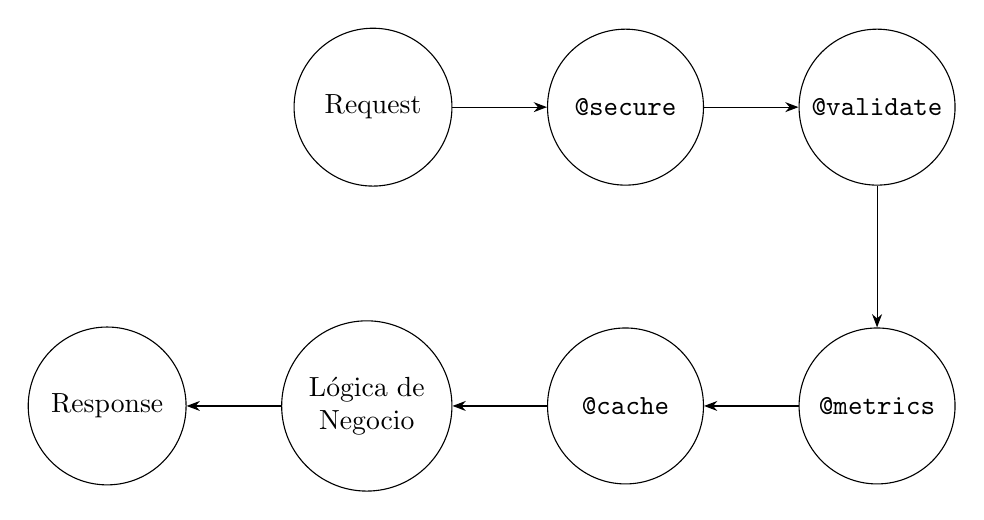
\begin{tikzpicture}[node distance=1.8cm and 1.2cm, auto, >=Stealth]
        % Fila superior
        \node[state] (req) {Request};
        \node[state, right=of req] (secure) {\texttt{@secure}};
        \node[state, right=of secure] (validate) {\texttt{@validate}};

        % Fila inferior (flujo de vuelta)
        \node[state, below=of validate] (metrics) {\texttt{@metrics}};
        \node[state, left=of metrics] (cache) {\texttt{@cache}};
        \node[state, left=of cache] (logic) {Lógica de\\Negocio};
        \node[state, left=of logic] (resp) {Response};

        % Conexiones
        \path[->] (req) edge (secure);
        \path[->] (secure) edge (validate);
        \path[->] (validate) edge (metrics);
        \path[->] (metrics) edge (cache);
        \path[->] (cache) edge (logic);
        \path[->] (logic) edge (resp);
    \end{tikzpicture}
    \vfill
    \begin{itemize}
        \item Un request HTTP es interceptado secuencialmente por cada decorador.
        \item Cada "aspecto" añade su comportamiento \textit{antes} o \textit{después} de ejecutar la lógica principal de la vista.
    \end{itemize}
\end{frame}

% ===================================================================
\section{Seguridad (\texttt{@secure})}
% ===================================================================

\begin{frame}{Aspecto de Seguridad: \texttt{@secure}}
    \begin{block}{Objetivo}
        Proteger rutas para que solo usuarios con roles específicos puedan acceder.
    \end{block}

    \begin{itemize}
        \item Se implementa como un decorador que recibe una lista de roles permitidos.
        \item Verifica el rol del usuario almacenado en la sesión (`g.user`).
        \item Si el usuario no tiene el rol adecuado, aborta la petición con un error HTTP 403 (Forbidden).
        \item Si no está logueado, se le redirige al login (manejado por \texttt{@login\_required}).
    \end{itemize}
\end{frame}

\begin{frame}[fragile]{Implementación del Decorador \texttt{@secure}}
    \begin{lstlisting}
def secure(roles=None):
    if roles is None: roles = []

    def decorator(view):
        @functools.wraps(view)
        def wrapped_view(**kwargs):
            if g.user is None:
                abort(401)  # Unauthorized
            
            if roles and g.user['role'] not in roles:
                abort(403)  # Forbidden

            print(f"Acceso concedido a {g.user['username']}")
            return view(**kwargs)
        return wrapped_view
    return decorator
    \end{lstlisting}
\end{frame}

% ===================================================================
\section{Cache y Métricas}
% ===================================================================

\begin{frame}{Aspectos de Cache y Métricas}
    \begin{block}{Objetivos}
        \begin{itemize}
            \item \texttt{@cache(ttl=60)}: Almacena el resultado de una vista en memoria para evitar recálculos costosos. El `ttl` (Time To Live) define la duración en segundos.
            \item \texttt{@metrics}: Mide y reporta el tiempo de ejecución de una vista. Es útil para identificar cuellos de botella.
        \end{itemize}
    \end{block}
    
    \begin{alertblock}{Orden de Aplicación}
        El orden de los decoradores importa. \texttt{@metrics} debe envolver a \texttt{@cache} para medir el tiempo real, incluyendo el acierto de caché.
    \end{alertblock}
\end{frame}

\begin{frame}[fragile]{Ejemplo de Uso en la Vista de Productos}
    \begin{lstlisting}
@bp.route('/')
@metrics
@cache(ttl=60)
def list_products():
    # ...
    \end{lstlisting}
\end{frame}

\begin{frame}[fragile]{Resultados en Consola}
    \textbf{Primer request (Cache Miss):}
    \begin{lstlisting}[language=bash]
METRICS for 'list_products':
  - Execution Time: 0.0028s
CACHE: Miss for key 'list_products:{}'. Caching result.
    \end{lstlisting}
    
    \vfill
    
    \textbf{Segundo request (Cache Hit):}
    \begin{lstlisting}[language=bash]
METRICS for 'list_products':
  - Execution Time: 0.0001s
CACHE: Hit for key 'list_products:{}'.
    \end{lstlisting}
\end{frame}

% ===================================================================
\section{Auditoría y Feature Flags}
% ===================================================================

\begin{frame}[fragile]{Auditoría (\texttt{@audit}) y Feature Flags (\texttt{@feature\_flag})}
    \begin{block}{\texttt{@audit(action='view\_order')}}
        Registra quién, qué y cuándo se realizó una acción.
    \end{block}
    \begin{lstlisting}
@audit(action='view_order')
def view_order(id): # ...
    \end{lstlisting}

    \begin{block}{\texttt{@feature\_flag('promo\_editor')}}
        Permite activar o desactivar funcionalidades en tiempo real.
    \end{block}
    \begin{lstlisting}
@feature_flag('promo_editor')
def manage_promotions(): # ...
    \end{lstlisting}
\end{frame}

% ===================================================================
\section{Validación con Pydantic}
% ===================================================================

\begin{frame}{Aspecto de Validación: \texttt{@validate\_with}}
    \begin{block}{Objetivo}
        Validar los datos de entrada (ej. formularios) de forma declarativa, separando las reglas de la lógica de la vista.
    \end{block}
    \begin{itemize}
        \item Se define un \textbf{esquema} con Pydantic que representa la estructura y reglas de los datos.
        \item El decorador \texttt{@validate\_with} intercepta el request, valida los datos contra el esquema y, si es exitoso, los adjunta al objeto `g` de Flask.
        \item Si la validación falla, muestra un error al usuario y detiene la ejecución.
    \end{itemize}
\end{frame}

\begin{frame}[fragile]{Paso 1: Definir el Esquema Pydantic}
    \begin{lstlisting}
// file: app/schemas.py
from pydantic import BaseModel, Field
from datetime import date

class PromotionSchema(BaseModel):
    name: str
    discount_percent: float = Field(
        ..., gt=0, lt=100,
        description="El descuento debe ser entre 0 y 100."
    )
    start_date: date
    end_date: date
    \end{lstlisting}
\end{frame}

\begin{frame}[fragile]{Paso 2: Aplicar el Decorador}
    \begin{lstlisting}
// file: app/promotions/routes.py
from app.schemas import PromotionSchema

@bp.route('/', methods=('GET', 'POST'))
@feature_flag('promo_editor')
@validate_with(PromotionSchema)
def manage_promotions():
    if request.method == 'POST':
        # No hay if/else de validacion!
        # Los datos ya estan validados en g.validated_data
        promo = g.validated_data
        db.execute(
            'INSERT INTO promotion ...',
            (promo.name, promo.discount_percent, ...)
        )
        # ...
    \end{lstlisting}
\end{frame}

% ===================================================================
\section{Demo Práctica y Conclusiones}
% ===================================================================

\begin{frame}{Demo: UI del Dashboard}
    \begin{columns}
        \begin{column}{0.5\textwidth}
            \textbf{Login de Usuario}\\
            \includegraphics[width=\textwidth]{example-image-a}
        \end{column}
        \begin{column}{0.5\textwidth}
            \textbf{Lista de Productos}\\
            \includegraphics[width=\textwidth]{example-image-b}
        \end{column}
    \end{columns}
    \tiny{\textit{Nota: Reemplazar con capturas de pantalla reales de la aplicación.}}
\end{frame}


\begin{frame}[fragile]{Cómo Ejecutar el Demo Local}
    \begin{block}{Pasos}
    \begin{enumerate}
        \item Clonar el repositorio y crear entorno virtual.
        \item Instalar dependencias:
        \begin{lstlisting}[language=bash]
uv pip install -r requirements.txt
        \end{lstlisting}
        \item Instalar el proyecto en modo editable (para que pytest funcione):
        \begin{lstlisting}[language=bash]
pip install -e .
        \end{lstlisting}
        \item Inicializar la base de datos (crea y puebla `project.sqlite`):
        \begin{lstlisting}[language=bash]
flask --app app init-db
        \end{lstlisting}
        \item Ejecutar la aplicación:
        \begin{lstlisting}[language=bash]
flask --app run
        \end{lstlisting}
        \item Acceder en \texttt{http://127.0.0.1:5000}.
            \begin{itemize}
                \item user: \texttt{admin}, pass: \texttt{admin} (acceso total)
                \item user: \texttt{featureuser}, pass: \texttt{password} (para ver feature flag)
            \end{itemize}
    \end{enumerate}
    \end{block}
\end{frame}

\begin{frame}{Ventajas y Conclusiones}
    \begin{itemize}
        \item<1-> \textbf{Código más limpio:} La lógica de negocio no se contamina con código de seguridad, cache, validación, etc.
        \item<2-> \textbf{Reutilización:} Los decoradores se pueden aplicar a cualquier vista con una sola línea.
        \item<3-> \textbf{Mantenibilidad:} Si se necesita cambiar la lógica de logging, solo se modifica el decorador \texttt{@audit}, no todas las vistas que lo usan.
        \item<4-> \textbf{Testabilidad:} Cada aspecto puede ser probado de forma aislada.
    \end{itemize}
    \vfill
    \begin{alertblock}{Conclusión Final}
        AOP, a través de decoradores en Python, es una herramienta poderosa para construir aplicaciones robustas, modulares y fáciles de mantener.
    \end{alertblock}
\end{frame}

\begin{frame}
    \begin{center}
        \Huge\bfseries ¿Preguntas?
    \end{center}
\end{frame}


\end{document} 